% Installation environnement de compilation et packages : 
% sudo apt-get install texlive-base texlive-lang-french texlive-latex-extra texlive-latex-recommended 
% Compilation :
% make

\let\pagebreakORIG\pagebreak
\let\clearpageORIG\clearpage
\let\cleardoublepageORIG\cleardoublepage

\ifx \removepagebreak \undefined
	\newcommand{\removepagebreak}{\renewcommand{\pagebreak}{}\renewcommand{\clearpage}{}\renewcommand{\cleardoublepage}{}}
\fi

\ifx \restorepagebreak \undefined
	\newcommand{\restorepagebreak}{\renewcommand{\pagebreak}{\pagebreakORIG}\renewcommand{\clearpage}{\clearpageORIG}\renewcommand{\cleardoublepage}{\cleardoublepageORIG}}
\fi

\documentclass[a4paper,titlepage]{scrreprt}
\usepackage[utf8]{inputenc}
\usepackage[francais]{babel}
\usepackage[T1]{fontenc}
\usepackage[babel=true]{csquotes}
\usepackage{graphicx}
\usepackage{float}
%\usepackage{listings}
%\usepackage{underscore}
\usepackage[bookmarks=true]{hyperref}
\hypersetup{
    %bookmarks=false,    % show bookmarks bar?
    pdftitle={Quidditch Manager 2014 : Software Requirement Document},    % title
    pdfauthor={Groupe 4},                     % author
    pdfsubject={Software Requirement Document of the videogame Quidditch Manager 2014},                        % subject of the document
    pdfkeywords={SRD, Quidditch, Manager}, % list of keywords
    colorlinks=true,       % false: boxed links; true: colored links
    linkcolor=blue,       % color of internal links
    citecolor=black,       % color of links to bibliography
    filecolor=black,        % color of file links
    urlcolor=purple,        % color of external links
    linktoc=page            % only page is linked
}%
\usepackage{makeidx} %pour l'index
\usepackage{glossaries} %pour le glossaire
\usepackage{scrhack}
\usepackage{array} %tableaux
\usepackage{xcolor} % Required for specifying custom colors
\usepackage{fix-cm} % Allows increasing the font size of specific fonts beyond LaTeX default specifications

%POUR LE TITRE :
\setlength{\oddsidemargin}{0mm} % Adjust margins to center the colored title box
\setlength{\evensidemargin}{0mm} % Margins on even pages - only necessary if adding more content to this template

\newcommand{\HRule}[1]{\hfill \rule{0.2\linewidth}{#1}} % Horizontal rule at the bottom of the page, adjust width here

\definecolor{grey}{rgb}{0.9,0.9,0.9} % Color of the box surrounding the title - these values can be changed to give the box a different color	

%Pour générer les fichiers pour makeIndex :
\makeindex
\makeglossaries

\begin{document}

\renewcommand{\glossaryname}{ }
\newglossaryentry{Quidditch}
{
  name=Quidditch,
  description={est un sport fictif issu de la saga
Harry Potter
créée par
J. K. Rowling.
Chaque équipe possède sept joueurs chevauchant des
balais volants. L'objectif étant de
marquer plus de points que l'adversaire en
marquant un maximum de buts et en
attrapant une balle magique, le
Vif d'or. Un match peut durer des mois et comporte des
risques mortels pour les joueurs}
}
\newglossaryentry{manager}
{
  name=manager,
  description={est l'utilisateur du programme, en charge de la gestion d'un club de Quidditch
  et de ses matchs}
}
\newglossaryentry{joueur}
{
  name=joueur,
  description={est un membre d'une équipe de Quidditch}
}
\newglossaryentry{match}
{
  name=match,
  description={est un affrontement de deux équipes de Quidditch sur un terrain}
}
\newglossaryentry{club}
{
  name=club,
  description={est un ensemble reprenant une équipe de Quidditch et son infrastructure}
}
\newglossaryentry{partie}
{
  name=partie,
  description={désigne la session de jeu que s'est créé l'utilisateur/Manager et qu'il peut gérer à sa guise. Il y a une partie par utilisateur}
}
\newglossaryentry{parcelle}
{
  name=parcelle,
  description={espace alloué à l'utilisateur où se trouvent ses bâtiments et son terrain de Quidditch}
}
\newglossaryentry{stade}
{
  name=stade,
  description={lieu sur l’espace alloué à un Manager où sont joués les matchs de Quidditch}
}
\newglossaryentry{terrain}
{
  name=terrain,
  description={espace à l'intérieur du stade où se déplacent les joueurs et les balles au cours d'un match}
}
\newglossaryentry{infirmerie}
{
  name=infirmerie,
  description={lieu où les joueurs du Managers sont soignés}
}
\newglossaryentry{centreentrainement}
{
  name=centre d’entrainement,
  description={lieu où le Manager peut faire s'entrainer ses joueurs}
}
\newglossaryentry{agencepublicite}
{
  name=agence de publicité,
  description={lieu où le Manager peut faire augmenter la popularité de ses joueurs}
}
\newglossaryentry{buvette}
{
  name=buvette,
  description={lieu où les supporters de l'équipe en déplacement pour un match qui ne se rendent pas sur place peuvent assister à une retransmission du match. Les consommations sont payantes et les bénéfices sont reversés au Manager}
}
\newglossaryentry{fanshop}
{
  name=fanshop,
  description={lieu où les supporters de l'équipe qui reçoit une équipe adverse pour un match peuvent acheter des produits dérivés}
}
\newglossaryentry{magasinbalais}
{
  name=magasin de balais,
  description={lieu où le Manager peut acheter/vendre des balais}
}
\newglossaryentry{centrerecrutement}
{
  name=centre de recrutement,
  description={lieu où le Manager peut acheter/vendre des joueurs}
}
\newglossaryentry{calendrier}
{
  name=calendrier,
  description={ensemble de rappels fixés dans le temps, le Manager est régulièrement rappelé à certaines actions (comme jouer un match) sur base de ce calendrier}
}

\newglossaryentry{evenement}
{
  name=événement,
  description={Action inscrite dans un calendrier qui rend possibles certains actions (jouer un match, sélectionner un joueur auparavant bloqué,...)}
}
\newglossaryentry{attrapeur}
{
  name=attrapeur,
  description={joueur dont la fonction au sein de l’équipe en cours de match est d’attraper le Vif d’Or}
}
\newglossaryentry{poursuiveur}
{
  name=poursuiveur,
  description={au nombre de 3 par équipe au cours d'un match, font des passes de Souafle entre eux et tentent de marquer des buts. Quand c'est l'équipe adverse qui a le souafle, ils essaient de le récupérer}
}
\newglossaryentry{batteur}
{
  name=batteur,
  description={au nombre de deux par équipe au cours d'un match. Un batteur frappe sur les Cognards et les envoie sur les joueurs adverses pour les blesser/déstabiliser}
}
\newglossaryentry{gardien}
{
  name=gardien,
  description={il n’y en a qu’un par équipe. Son rôle est d’empêcher les Poursuiveurs de l’équipe adverse de marquer des buts en interceptant leurs tirs}
}
\newglossaryentry{souafle}
{
  name=souafle,
  description={balle inerte unique manipulée pendant un match par les Poursuiveurs à travers des passes et des tentatives de tirs dans l’un des cercles d’or pour marquer un but}
}
\newglossaryentry{cognard}
{
  name=cognard,
  description={au nombre de deux. Plus petite que le Souafle. Balle magique qui essaie de frapper les joueurs pour les faire tomber de leur balais. Ces balles sont cognées par les batteurs pour les diriger vers les joueurs adverses}
}
\newglossaryentry{vifOr}
{
  name=vif d’Or,
  description={petite balle unique ayant sa propre volonté, qui se déplace aléatoirement et très rapidement dans les airs. Lorsqu’un Attrapeur attrape le Vif d’Or, la partie s’achève}
}

\renewcommand{\indexname}{4 Index}




\thispagestyle{empty} % Remove page numbering on this page

%----------------------------------------------------------------------------------------
%	TITLE SECTION
%----------------------------------------------------------------------------------------

\colorbox{grey}{
	\parbox[t]{1.0\linewidth}{
		\centering \fontsize{50pt}{80pt}\selectfont % The first argument for fontsize is the font size of the text and the second is the line spacing - you may need to play with these for your particular title
		\vspace*{0.7cm} % Space between the start of the title and the top of the grey box
		
		\hfill SOFTWARE REQUIREMENTS \\
		\hfill DOCUMENT \\
		\hfill Quidditch Manager 2014\par
		
		\vspace*{0.7cm} % Space between the end of the title and the bottom of the grey box
	}
}

%----------------------------------------------------------------------------------------

\vfill % Space between the title box and author information

%----------------------------------------------------------------------------------------
%	AUTHOR NAME AND INFORMATION SECTION
%----------------------------------------------------------------------------------------

{\centering \large 
\hfill Groupe 4 : Manon Legrand, Hélène Plisnier, Audry Delestree, David Bertha \\
\hfill INFOF209 \\
\hfill Université Libre de Bruxelles \\
\hfill Version 1.0 \\

\HRule{1pt}} % Horizontal line, thickness changed here

%----------------------------------------------------------------------------------------

\clearpage % Whitespace to the end of the page

\tableofcontents
\chapter{Introduction}
\section{But du projet}
  % Texte (d’une demi-page approximativement) décrivant les tenants
  % et aboutissants du projet, et énumérant les différents types de
  % personnes qui vont bénéficier de la réalisation du projet.
  Le \gls{Quidditch}\index{Quidditch} \gls{manager}\index{manager} est un jeu multi-joueurs de gestion
  et de stratégie, se jouant par réseau.
  Un manager (l'utilisateur) gère son équipe de \gls{joueur}s, qu'il peut entrainer
  au travers des bâtiments construits sur la \index{parcelle}parcelle qui lui est attribuée. Certains de ces bâtiments permettent aussi de faire des achats et des ventes de balais ou de joueurs.
  Le but pour le manager est de déveloper son \gls{club} aussi bien au niveau commercial
  que sportif.
  À travers la construction et l'évolution de ses bâtiments, le manager ouvre et
  augmente des possibilités de gestion du club, notamment la possibilité
  d'améliorer les caractéristiques de ses joueurs, ces caractéristiques
  étant déterminantes dans le déroulement d'un match.
  Les différents managers sont périodiquement invités à s'affronter par
  ces \gls{match}s s'inscrivant dans un championnat, étalonné dans le temps. 
  
  Ces matchs se déroulent
  dans un stade propre à un des managers et apportent une entrée d'argent
  dûe notamment à la victoire d'une équipe mais aussi au nombre de tickets vendus.
  Au cours du match, les managers en présence choisissent à chaque tour de jeu
  des déplacements pour leurs différents joueurs. Il existe quatre fonction possible
  pour un joueur lors d'un match. Un joueur peut être un \gls{attrapeur}\index{joueur!attrapeur}, un \gls{batteur}\index{joueur!batteur}, un \gls{gardien}\index{joueur!gardien}
  ou un \gls{poursuiveur}\index{joueur!poursuiveur}.
  Chacun de ces rôles implique des actions possibles différentes au cours du match.
  Mais il est possible à chacun de se déplacer sur le terrain, celui-ci étant représenté par
  des hexagones (il y a donc 6 directions de déplacement possibles à partir d'une case).
  De plus, les joueurs se partagent le terrain avec les différentes balles du jeu, 
  qu'ils devront manipuler selon les règles pour emmener leur équipe vers la victoire,
  celle-ci étant déterminée lorsque le \gls{vifOr} est attrapé ou par abandon.


\section{Historique du document}
  % Tableau reprenant tous les changements effectués sur le
  % document. Chaque ligne de celui-ci contiendra les champs
  % suivants : numéro de version, auteur et date de la modification,
  % description des changements. Le tableau sera trié de manière
  % décroissante sur le numéro de version.
  \begin{tabular}{|c|c|c|c|}
    \hline
    Numéro de version & Auteur & Date de la modification & Description des changements \\
    \hline
    0.1 & David & 13/12/13 & Squelette du code \LaTeX \\
    0.2 & Hélène & 19/12/13 & Première ébauche de la section 2.1 \\
    0.3 & Manon & 20/12/13 & Section 2.1 finale \\
    0.4 & David & 20/12/13 & Sections 1,  2.2 et 2.3 \\
    0.5 & Manon & 20/12/13 & Section 3.1 \\
    0.5 & David & 20/12/13 & Section 3.2 \\
    0.6 & Audry & 20/12/13 & Section 3.3 \\
    0.7 & David & 20/12/13 & Glossaire et Index \\
    1.0 & Manon & 20/12/13 & Relecture et révision \\
    1.1 & Hélène & 07/02/14 & 1ère correction \\
    \hline
  \end{tabular}


\section{Glossaire}
  % Définition des termes, des acronymes et des abréviations
  % utilisés dans le présent document.
  \removepagebreak
  \printglossaries
  \restorepagebreak
\chapter{Besoins de l'utilisateur}
  % Cette deuxième section reprend les services que le système doit
  % fournir aux utilisateurs, ainsi que les contraintes de
  % fonctionnement du système. Elle doit être complète et consistante,
  % et il faut qu’elle soit rédigée dans un langage spécialement
  % compréhensible pour le client, c’est-à-dire en évitant entre autres
  % tout terme ou détail techniques.
  
  
\section{Exigences fonctionnelles}
  % Ce type d’exigences sera décrit en utilisant des diagrammes use
  % case et en fournissant une description pour chacun d’entre eux
  % (comme vu au cours théorique et aux exercices).
  
  Les cas d'utilisation présentés ci-dessous décrivent les différentes actions proposées au client par le programme.

  \subsection{Cas d'utilisation 1: démarrer le jeu}
  \begin{figure}[H]
    \center
    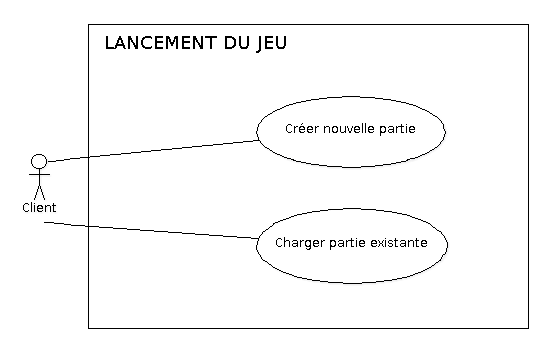
\includegraphics[scale=0.5]{uml/useCaseView/Lancementdujeu.png}
    \caption{Cas d'utilisation 1: Démarrer le jeu}
  \end{figure}	
    L'utilisateur démarre le jeu. Soit il a déjà commencé une \gls{partie}\index{partie}; dans ce cas, l'utilisateur s'identifie et reprend sa partie là où il l'avait laissée. \\
    Soit il ne possède pas encore de partie; le programme lui demande alors quelques informations d'identification. 
    Il se voit ensuite attribuer une équipe de 7 \gls{joueur}s médiocres et une \gls{parcelle}\index{parcelle}. 
    Au commencement, ce dernier est presque désert, composé uniquement d'un 
    \gls{stade}\index{bâtiment!Stade} de \gls{Quidditch}\index{Quidditch} et d'emplacements vides prévus pour accueillir les bâtiments.
    \subsubsection{Créer nouvelle partie}
      \begin{itemize}
        \item \textbf{Relations avec d'autres cas d'utilisation}  : Néant.
        \item \textbf{Pré-conditions} : Le client désire se créer une nouvelle partie.
        \item \textbf{Post-conditions} : Le client possède une partie.
        \item \textbf{Cas général} : Le client veut créer une nouvelle partie. Il devra alors rentrer toute une série d’informations concernant cette partie nécessaire à l’identification de cette partie et au bon fonctionnement du jeu (nom du \index{manager}manager, nom de l’équipe, mot de passe, etc.)
        \item \textbf{Cas exceptionnels} :
          \begin{itemize}
            \item Un manager avec le nom indiqué par le client existe déjà. Le programme le signale au client et lui demande d'entrer un autre nom. Ceci termine ce use case.
          \end{itemize}
      \end{itemize}
    \subsubsection{Charger partie existante}
      \begin{itemize}
        \item \textbf{Relations avec d'autres cas d'utilisation}  : Néant.
        \item \textbf{Pré-conditions} : Il faut qu’il existe déjà une partie à laquelle créée par ce client.
        \item \textbf{Post-conditions} : Le client a accès à sa partie.
        \item \textbf{Cas général} : Le client souhaite continuer une partie déjà entamée et rentre le nom de la partie ainsi que le mot de passe pour récupérer les informations concernant cette partie.
        \item \textbf{Cas exceptionnels} :
          \begin{itemize}
            \item Il n’y a pas de partie existante. Le programme le signale au client et lui propose de se créer une nouvelle partie. Ceci termine ce use case.
			\item L’identification de la partie a échoué (mauvais nom ou mot de passe). Le programme le signale au client et lui redemande d'entrer le nom de la partie ainsi que le mot de passe. Ceci termine ce use case.
          \end{itemize}
      \end{itemize}

  \subsection{Cas d'utilisation 2: jouer un match}
    \begin{figure}[H]
    \center
    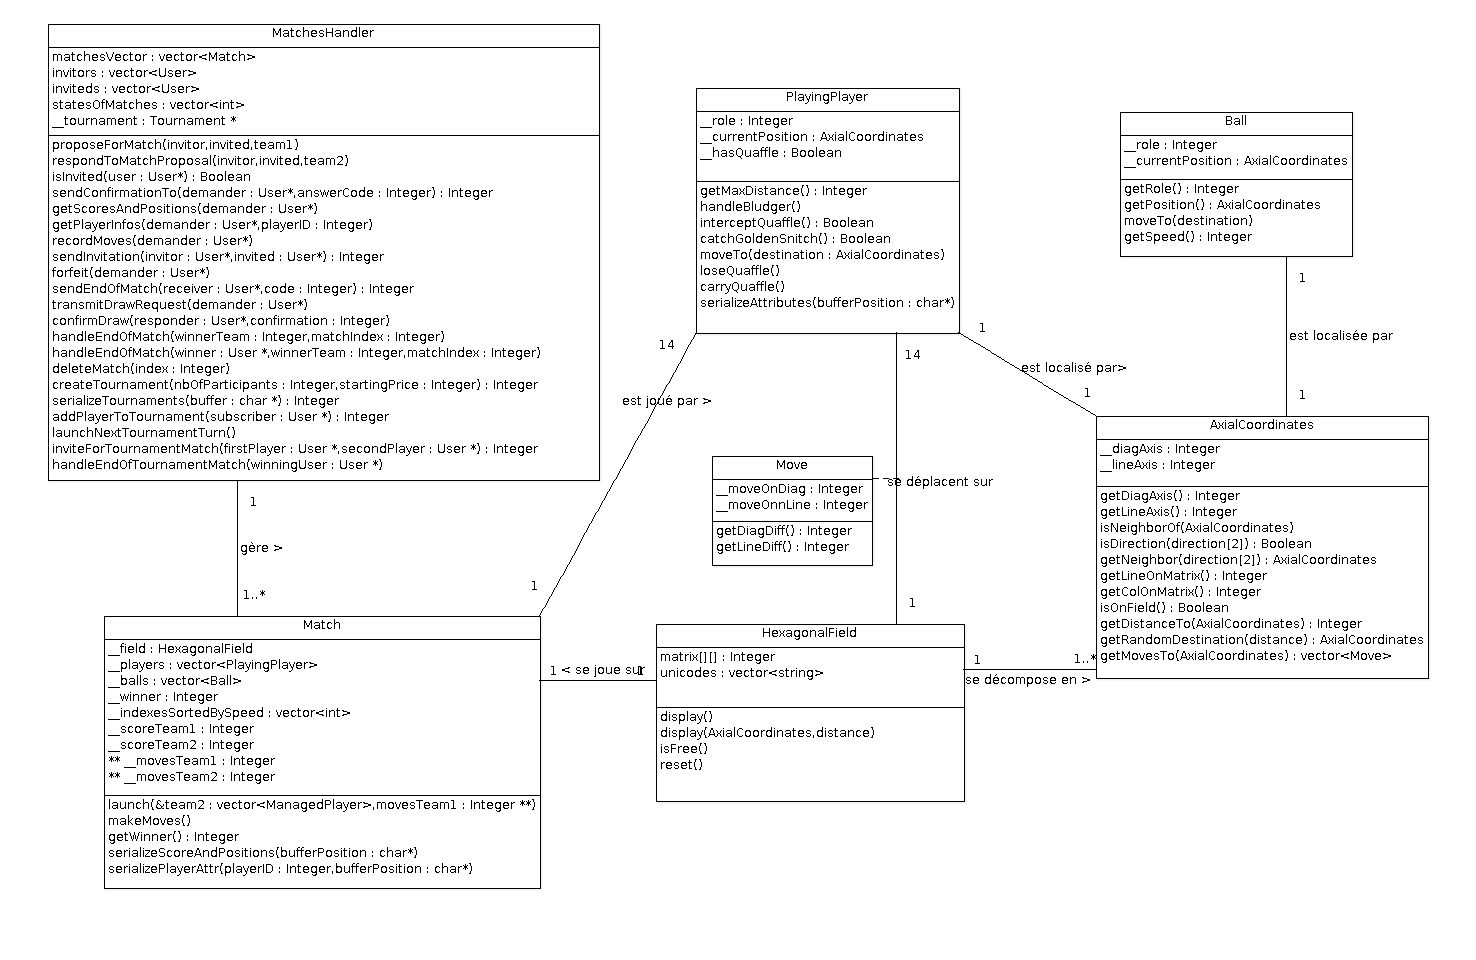
\includegraphics[scale=0.4]{uml/useCaseView/Match.png}
    \caption{Cas d'utilisation 2: Jouer un match}
  \end{figure}	
    Tous les X temps, le Manager\index{manager} est invité à affronter un Manager adverse dans un \gls{match}\index{match} soit à
    domicile, soit à l'extérieur (cette information déterminera à qui reviendront les recettes
    générées par la vente de tickets). Avant de commencer le match proprement dit,
    le Manager doit choisir sept de ses joueurs pour former son équipe. 
    Une fois le match terminé, le Manager prend connaissance du résultat du match 
    (s'il a gagné ou perdu) et des recettes éventuellement réalisées. Un match peut être amical (démarré à la suite d'une invitation pouvant être envoyée à tout moment par un Manager à un autre Manager connecté) ou s'inscrivant dans un championnat. Les deux types de match ont pour point commun de rendre le Manager gagnant plus riche d'au moins une prime de victoire.

    \subsubsection{Exécuter un tour}
      \begin{itemize}
        \item \textbf{Relations avec d'autres cas d'utilisation}  : Est étendu par Déplacer un joueur et Faire une action particulière
        \item \textbf{Pré-conditions} : L'action se déroule lors d'un match.
        \item \textbf{Post-conditions} : Un tour a été effectué et chaque joueur sur le terrain a (éventuellement) bougé.
        \item \textbf{Cas général} : Un match se déroule tour par tour. À chaque tour, les clients qui s’affrontent doivent indiquer, pour chaque joueur, un mouvement à effectuer ou simplement les laisser sur place.
        \item \textbf{Cas exceptionnels} :
          \begin{itemize}
            \item L’adversaire s’est déconnecté et ne s’est pas reconnecté dans le temps imparti. Le programme signale la déconnexion inopinée et le match s’arrête.
          \end{itemize}
      \end{itemize}
    \subsubsection{Déplacer un joueur}
      \begin{itemize}
        \item \textbf{Relations avec d'autres cas d'utilisation}  : Etend Exécuter un tour
        \item \textbf{Pré-conditions} : Le joueur sélectionné pour faire un déplacement n’a pas été choisi pour une action particulière.
        \item \textbf{Post-conditions} : Le joueur sélectionné a été déplacé ou est resté sur place.
        \item \textbf{Cas général} : Le client sélectionne un joueur et choisit où celui-ci doit se déplacer sur le terrain\index{terrain} ou le laisse sur place. Le client est informé de l’ensemble des destinations possibles pour le joueur sélectionné.
        \item \textbf{Cas exceptionnels} : 
        \begin{itemize}
            \item Le Manager ne choisi aucune direction pour le joueur sélectionné. Le joueur reste donc sur place.
          \end{itemize}
      \end{itemize}
    \subsubsection{Faire une action particulière}
      \begin{itemize}
        \item \textbf{Relations avec d'autres cas d'utilisation}  : Etend Exécuter un tour. Généralise Faire une passe, Tirer aux buts et Frapper cognard
        \item \textbf{Pré-conditions} : Aucune action particulière n'a encore été assignée au joueur sélectionné.
        \item \textbf{Post-conditions} : Le joueur a une action particulière à accomplir.
        \item \textbf{Cas général} : Le client choisit le joueur et l’action que celui-ci doit réaliser. Cette action dépend du poste du joueur.
        \item \textbf{Cas exceptionnels} : Néant.
      \end{itemize}
    \subsubsection{Faire une passe}
      \begin{itemize}
        \item \textbf{Relations avec d'autres cas d'utilisation}  : Spécialise Faire une action particulière
        \item \textbf{Pré-conditions} : Le joueur qui va faire la passe doit tenir le \gls{souafle}\index{balle!souafle} et doit être un \gls{poursuiveur}s \index{joueur!poursuiveur}.
        \item \textbf{Post-conditions} : Que la passe soit réussie ou ratée, le joueur ne possèdera plus le souafle.
        \item \textbf{Cas général} : Le client choisit l’endroit de destination de la passe. Les endroits possibles dépendent des compétences du joueur qui a le souafle. Attraper le souafle suite à une passe ou l’intercepter (passe adverse) se fait de façon automatique par un poursuiveur se trouvant sur la trajectoire de la passe.
        \item \textbf{Cas exceptionnels} :
        \begin{itemize}
            \item Le joueur est heurté par un \gls{cognard}\index{balle!cognard}. La passe échoue. 
          \end{itemize}
      \end{itemize}
     \subsubsection{Tirer aux buts}
      \begin{itemize}
        \item \textbf{Relations avec d'autres cas d'utilisation}  : Spécialise Faire une action particulière
        \item \textbf{Pré-conditions} : Le poursuiveur qui veut tirer doit tenir le souafle et se trouver dans l’alignement d’un des buts. 
        \item \textbf{Post-conditions} : Qu’il y ait but ou non, le joueur ne tiendra plus le souafle.
        \item \textbf{Cas général} : Le client essaie de marquer un but en indiquant au poursuiveur détenant le souafle vers quel but il doit tirer. Intercepter le souafle se fait automatiquement par le \gls{gardien}\index{joueur!gardien} ou les \gls{poursuiveur}s \index{joueur!poursuiveur} adverses s’ils se trouvent sur la trajectoire du souafle. Si le tir est réussi, l'équipe qui vient de marquer gagne 10 points.
        \item \textbf{Cas exceptionnels} :
        \item Le poursuiveur qui s'apprête à tirer est heurté par un \gls{cognard}\index{balle!cognard}. Le tir au but échoue. 
          %\end{itemize}
      \end{itemize}
    \subsubsection{Frapper cognard}
      \begin{itemize}
        \item \textbf{Relations avec d'autres cas d'utilisation}  : Spécialise Faire une action particulière
        \item \textbf{Pré-conditions} : Le joueur qui va essayer de frapper un \gls{cognard}\index{balle!cognard} doit être un batteur\index{joueur!batteur} et doit se situer près du cognard.
        \item \textbf{Post-conditions} : Le cognard est projeté dans la direction voulue.
        \item \textbf{Cas général} : Le client indique dans quelle direction le batteur doit frapper le cognard.
        \item \textbf{Cas exceptionnels} : 
        \item Le batteur rate son coup. Le cognard heurte le joueur.
      \end{itemize}
    \subsubsection{Finir le match}
      \begin{itemize}
        \item \textbf{Relations avec d'autres cas d'utilisation}  : Généralise Attraper \gls{vifOr}\index{balle!Vif d'Or} et Déclarer forfait
        \item \textbf{Pré-conditions} : Cette action se déroule lors d'un match.
        \item \textbf{Post-conditions} : Il y a un club gagnant et un club perdant ou deux ex-aequos.
        \item \textbf{Cas général} : Le match va se terminer, le score est figé et les résultats vont déterminer ce que va gagner ou perdre (argent, popularité) chaque manager\index{manager}.
        \item \textbf{Cas exceptionnels} :
          \begin{itemize}
            \item Le match se finit parce que les deux clients qui s’affrontent se sont déconnectés et n’ont pas joué le match jusqu’au bout. Le match est considéré comme annulé.
            \item Si les 7 joueurs d'une même équipe sont blessés et ne peuvent continuer à jouer, l'équipe adverse gagnera le match. Les joueurs blessés sont envoyés à l'infirmerie et sont bloqués jusqu'à leur rétablissement.
          \end{itemize}
      \end{itemize}
    \subsubsection{Attraper vif d'or}
      \begin{itemize}
        \item \textbf{Relations avec d'autres cas d'utilisation}  : Spécialise Finir le match
        \item \textbf{Pré-conditions} : Un des \gls{attrapeur}s \index{joueur!attrapeur} a repéré le \gls{vifOr}.
        \item \textbf{Post-conditions} : Si l'attrapeur réussit son coup, le match est terminé. S'il échoue, le match continue.
        \item \textbf{Cas général} : Un des attrapeurs a repéré le vif d’or, c’est-à-dire qu’en se déplaçant sur le terrain\index{terrain}, il est arrivé suffisamment proche du vif d’or pour que sa précision permette de le repérer (et de le rendre visible pour son Manager). L’attrapeur essaiera automatiquement de l’attraper (la réussite de l’action dépend des qualités de l’attrapeur et de sa distance par rapport au vif d’or). S’il réussit à l’attraper, son équipe gagne 150 points et le match est terminé.
        \item \textbf{Cas exceptionnels} :
         \begin{itemize}
            \item L'attrapeur est heurté par un cognard. Le vif d'or reste libre.
            \end{itemize}
      \end{itemize}
    \subsubsection{Déclarer forfait}
      \begin{itemize}
        \item \textbf{Relations avec d'autres cas d'utilisation}  : Spécialise Finir match
        \item \textbf{Pré-conditions} : L'action se déroule au cours d'un match.
        \item \textbf{Post-conditions} : Le match est terminé. Le Manager qui n'a pas déclaré forfait a gagné.
        \item \textbf{Cas général} : Un des Managers souhaite mettre fin au match en déclarant forfait (équivaut à une défaite 150-0, peu importe le score lorsqu’il déclare forfait).
        \item \textbf{Cas exceptionnels} :
          \begin{itemize}
            \item Si un Manager se déconnecte au cours d’un match et ne se reconnecte pas dans un certain délai de temps, on considérera qu’il a déclaré forfait.
          \end{itemize}
      \end{itemize}


  \subsection{Cas d'utilisation 3: gérer ses bâtiments}
    \begin{figure}[H]
    \center
    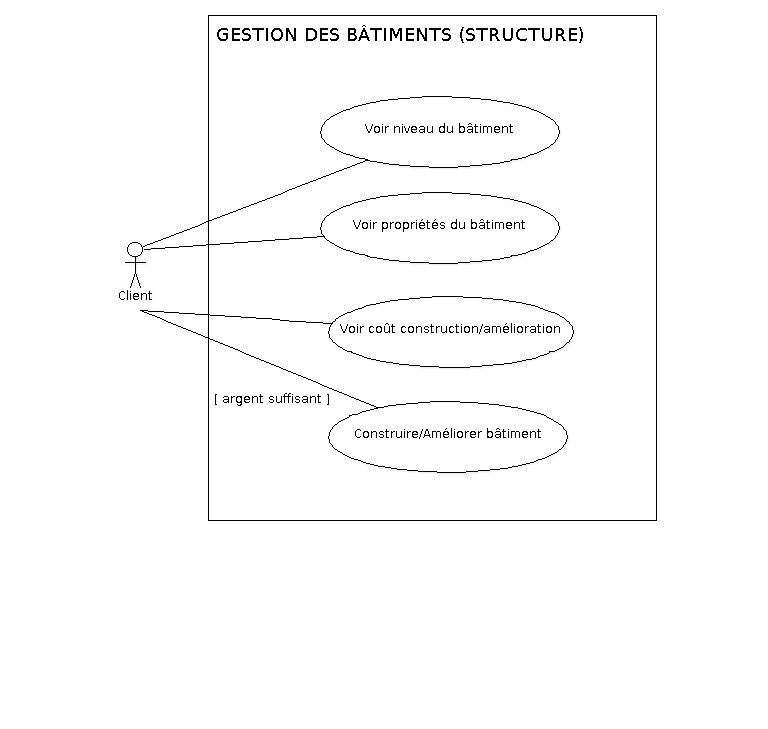
\includegraphics[scale=0.5]{uml/useCaseView/Gestiondesbatimentsstructure.png}
    \caption{Cas d'utilisation 3: Gérer ses bâtiments}
  \end{figure}	
  Différents bâtiments sont disponibles à la construction pour le Manager, \index{manager}
  moyennant un certain coût et un temps d'attente (avant fin des travaux). 
  Généralement: une fois construits, le Manager peut améliorer ses bâtiments 
  et accéder aux informations les concernant. Certains bâtiments offrent 
  des usages supplémentaires.
    \subsubsection{Voir niveau du bâtiment}
      \begin{itemize}
        \item \textbf{Relations avec d'autres cas d'utilisation}  : Néant.
        \item \textbf{Pré-conditions} : On a sélectionné un bâtiment.
        \item \textbf{Post-conditions} : Néant.
        \item \textbf{Cas général} : Le client souhaite savoir quel est le niveau actuel (de construction et d'amélioration) d’un certain bâtiment. 
        \item \textbf{Cas exceptionnels} : Néant.
      \end{itemize}
    \subsubsection{Voir propriétés du bâtiment}
      \begin{itemize}
        \item \textbf{Relations avec d'autres cas d'utilisation}  : Néant.
        \item \textbf{Pré-conditions} : On a sélectionné un bâtiment.
        \item \textbf{Post-conditions} : Néant.
        \item \textbf{Cas général} : Le client souhaite voir les propriétés d’un certain bâtiment (ces propriétés dépendent du niveau et du bâtiment).
        \item \textbf{Cas exceptionnels} :
          \begin{itemize}
            \item Le bâtiment est de niveau 0, il n'a pas encore été construit et n'a donc actuellement pas de propriétés effectives.
          \end{itemize}
      \end{itemize}
    \subsubsection{Voir coût construction/amélioration}
      \begin{itemize}
        \item \textbf{Relations avec d'autres cas d'utilisation}  : Néant.
        \item \textbf{Pré-conditions} : On a sélectionné un bâtiment.
        \item \textbf{Post-conditions} : Néant.
        \item \textbf{Cas général} : Le client souhaite connaître la somme requise pour pouvoir lancer un projet de construction ou d’amélioration d’un certain bâtiment.
        \item \textbf{Cas exceptionnels} : Néant.
      \end{itemize}
    \subsubsection{Construire/Améliorer bâtiment}
      \begin{itemize}
        \item \textbf{Relations avec d'autres cas d'utilisation}  : Néant.
        \item \textbf{Pré-conditions} : Le Manager possède suffisamment d’argent pour payer le projet de construction ou d’amélioration. Le Manager a choisi le bâtiment qu’il désire améliorer.
        \item \textbf{Post-conditions} : Le projet sera terminé après un certain laps de temps déterminé par le niveau du bâtiment. La date de fin des travaux est sauvegardée dans un \gls{calendrier}\index{calendrier} qui sera vérifié régulièrement.
        \item \textbf{Cas général} : Le Manager souhaite construire (si niveau actuel vaut 0) ou améliorer (si niveau actuel vaut 1 ou plus) un certain bâtiment et choisit donc de lancer un projet de construction/amélioration. Le coût des travaux est déduit de son capital et les travaux ne sont achevés qu'après un certain temps.
        \item \textbf{Cas exceptionnels} :
        \begin{itemize}
            \item Le bâtiment sélectionné est à son niveau maximum. Aucune évolution supplémentaire ne peut être effectuée sur ce bâtiment.
          \end{itemize}
      \end{itemize}

  \subsection{Cas d'utilisation 4: gérer son équipe}
  \begin{figure}[H]
    \center
    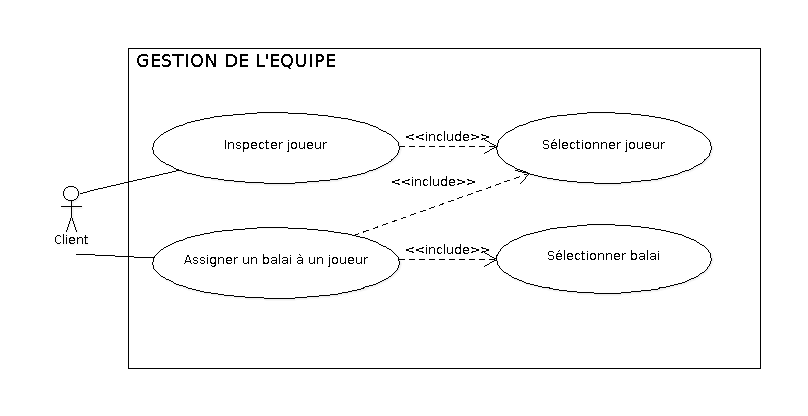
\includegraphics[scale=0.5]{uml/useCaseView/Gestiondelequipe.png}
    \caption{Cas d'utilisation 4: gérer son équipe}
  \end{figure}	
  Le manager\index{manager} a une vue sur tous les joueurs de son \gls{club} ; \index{club} 
  leur description et leurs caractéristiques. 
  Il lui est également donné la possibilité d'assigner un nouveau balai à tel ou tel joueur.
    \subsubsection{Inspecter joueur}
      \begin{itemize}
        \item \textbf{Relations avec d'autres cas d'utilisation}  : Inclut Sélectionner joueur
        \item \textbf{Pré-conditions} : Le Manager a sélectionné un de ses joueurs.
        \item \textbf{Post-conditions} : Néant.
        \item \textbf{Cas général} : Le client souhaite se renseigner sur les capacités d’un de ses joueurs. Il pourra voir le niveau de chaque attribut du joueur ainsi que sa popularité et son balai.

        \item \textbf{Cas exceptionnels} : Néant.
      \end{itemize}
    \subsubsection{Assigner un balai à un joueur}
      \begin{itemize}
        \item \textbf{Relations avec d'autres cas d'utilisation}  : Inclut Sélectionner joueur et Sélectionner balai
        \item \textbf{Pré-conditions} : Le Manager a sélectionné un balai disponible pour une assignation.
        \item \textbf{Post-conditions} : Le balai sélectionné est assigné au joueur. L’ancien balai est à nouveau disponible pour une assignation.
        \item \textbf{Cas général} : Le Manager souhaite changer le balai d’un joueur. Les balais ont des bonus particuliers qui permettent d’augmenter certains attributs des joueurs. Une fois u'un joueur s'est vu assigné un nouveau balai, l'ancien n'est plus assigné à aucun joueur mais reste disponible.
        \item \textbf{Cas exceptionnels} :
          \begin{itemize}
            \item Le Manager retire le balai d’un joueur sans lui en assigner un nouveau s’il n'a pas au préalable sélectionné de balai disponible.
          \end{itemize}
      \end{itemize}
    \subsubsection{Sélectionner joueur}
      \begin{itemize}
        \item \textbf{Relations avec d'autres cas d'utilisation}  :  Est inclus dans Inspecter joueur et Assigner un balai à un joueur
        \item \textbf{Pré-conditions} : Le Manager a une vue sur tous ses joueurs.
        \item \textbf{Post-conditions} : Le Manager a accès aux caractéristiques propres au joueur sélectionné.
        \item \textbf{Cas général} : Le client choisit le joueur qu’il veut gérer (inspecter ou changer le balai).
        \item \textbf{Cas exceptionnels} : Néant.
      \end{itemize}
    \subsubsection{Sélectionner balai}
      \begin{itemize}
        \item \textbf{Relations avec d'autres cas d'utilisation}  : Est inclus dans Assigner un balai à un joueur
        \item \textbf{Pré-conditions} : \index{balai}Le balai doit être disponible, c’est-à-dire qu’il ne doit être assigné à aucun joueur.
        \item \textbf{Post-conditions} : Le balai disponible est sélectionné.
        \item \textbf{Cas général} : Le client choisit le balai qu’il va assigner à un joueur. Une fois assigné, le balai ne sera plus disponible.
        \item \textbf{Cas exceptionnels} : Néant.
      \end{itemize}

  \subsection{Cas d'utilisation 5: magasins}
  \begin{figure}[H]
    \center
    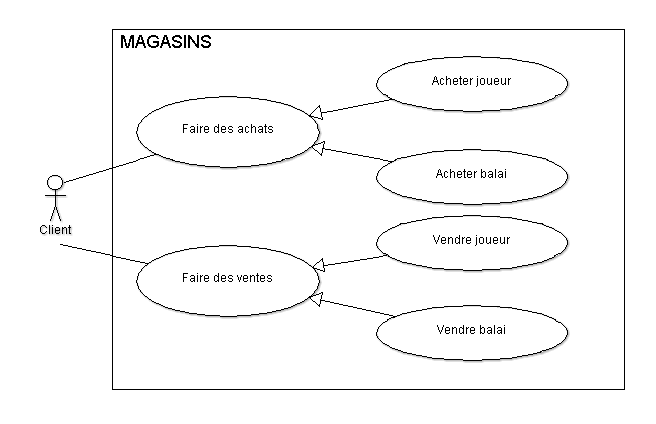
\includegraphics[scale=0.5]{uml/useCaseView/Magasins.png}
    \caption{Cas d'utilisation 5: Magasins}
  \end{figure}
  Dans le bâtiment \enquote{\gls{centrerecrutement}} \index{bâtiment!Centre de Recrutement}, le Manager pourra "s'offrir" de nouveaux joueurs, 
  selon ses moyens. Il peut également vendre les joueurs qu'il possède. Les joueurs sont vendus aux enchères. Le vendeur décide du prix de vente dans une fourchette de prix (estimée d'après les capacités du joueur).
  Dans le bâtiment \enquote{\gls{magasinbalais}} \index{bâtiment!Magasin de balais}, le Manager pourra acheter ou vendre des balais.\index{balai} Outre les balais de base qui permettent juste de voler, 
  il y a aussi des balais qui octroient des bonus à certaines capacités des joueurs.
    \subsubsection{Faire des achats}
      \begin{itemize}
        \item \textbf{Relations avec d'autres cas d'utilisation}  : Généralise Acheter joueur et Acheter balai
        \item \textbf{Pré-conditions} : Le Manager doit posséder suffisamment d’argent pour payer ce qu’il veut acheter. Le Manager doit avoir de la place pour un joueur ou pour un balai.
        \item \textbf{Post-conditions} : Le prix est déduit du solde du manager. L'item se trouve en la possession du Manager.
        \item \textbf{Cas général} : Le client souhaite acheter un nouveau joueur pour renforcer son équipe ou un nouveau balai pour renforcer un joueur.
        \item \textbf{Cas exceptionnels} : Néant.
      \end{itemize}
    \subsubsection{Faire des ventes}
      \begin{itemize}
        \item \textbf{Relations avec d'autres cas d'utilisation}  : Généralise Vendre joueur et Vendre balai.
        \item \textbf{Pré-conditions} :
        \begin{itemize}
            \item Le Manager a choisit le joueur ou le balai qu'il désire vendre.
            \item L'item que le Manager désire vendre doit être disponible. S'il s'agit d'un balai, il ne peut être assigné à un joueur lors de sa mise en vente. S'il s'agit d'un joueur, il doit être libre (non bloqué par une blessure, un entraînement ou une tournée de promotion).
        \end{itemize}    
        \item \textbf{Post-conditions} : Le Manager reçoit l’argent de la vente. Il ne possède plus l'item vendu. L'item devient disponible à l'achat.
        \item \textbf{Cas général} : Le Manager souhaite vendre un joueur ou un balai s’il n’en a plus besoin ou si ses finances vont mal. \index{balai}\index{joueur}
        \item \textbf{Cas exceptionnels} : Néant.
      \end{itemize}
    \subsubsection{Acheter joueur}
      \begin{itemize}
        \item \textbf{Relations avec d'autres cas d'utilisation}  : Spécialise Faire des achats
        \item \textbf{Pré-conditions} : Le Manager s'est manifesté en sélectionnant le joueur qui l'intéresse dans la liste des joueurs mis en vente.
        \item \textbf{Post-conditions} : S'il est le seul enchérisseur, le Manager remporte l'enchère. S'ils sont plusieurs à enchérir, le Manager peut participer au tour suivant. Si personne n'enchérit au tour suivant et que le Manager était le dernier enchérisseur du tour courant, il remporte l'enchère. Sinon, le Manager n'a pas remporté l'enchère.
        \item \textbf{Cas général} : Le client choisit le joueur qu’il veut acheter selon les capacités de ce dernier (ce qui l’intéresse), et selon le prix de ce joueur. Les joueurs achetés sont équipés d'un balai médiocre qui n'a pas de valeur financière. Les enchères se déroulent par tours. Le Manager manifeste son intérêt en se signalant au premier tour. Il assure ainsi sa participation au tour suivant. Si le prix du joueur devient trop élevé à son goût, le Manager peut abandonner en ne renouvellant pas son enchère lors d'un tour, ce qui lui interdira de surenchérir lors du tour suivant.
        \item \textbf{Cas exceptionnels} :
        \begin{itemize}
            \item Personne ne se manifeste au premier tour. La vente est annulée, le joueur retourne en la possession du vendeur.
            \item Un Manager souhaite surenchérir alors que le prix, augmenté de son enchère, est au-dessus de ses moyens. Le programme le lui signale et son offre n'est pas prise en compte.
            \item Un Manager désire surenchérir alors qu'il n'a pas émis d'enchère au tour précédant. Le programme le lui signale et ne considère pas son offre.
          \end{itemize}
      \end{itemize}
    \subsubsection{Acheter balai}
      \begin{itemize}
        \item \textbf{Relations avec d'autres cas d'utilisation}  : Spécialise Faire des achats
        \item \textbf{Pré-conditions} : Néant.
        \item \textbf{Post-conditions} : Néant.
        \item \textbf{Cas général} : Le client choisit le balai qu’il veut acheter en fonction des caractéristiques de celui-ci et de son prix. \index{balai}
        \item \textbf{Cas exceptionnels} :
          \begin{itemize}
            \item Des balais médiocres sans bonus sont disponibles gratuitement.
          \end{itemize}
      \end{itemize}
    \subsubsection{Vendre joueur}
      \begin{itemize}
        \item \textbf{Relations avec d'autres cas d'utilisation}  : Spécialise Faire des ventes
        \item \textbf{Pré-conditions} : Néant.
        \item \textbf{Post-conditions} : Néant.
        \item \textbf{Cas général} : Le client choisit le joueur qu’il veut vendre et à quel prix (entre des bornes supérieure et inférieure imposées). Le joueur ne sera plus dans l’équipe mais sera disponible à l’achat. Le client peut vendre aux enchères un joueur équipé d’un balai, ce qui augmente un peu la valeur du joueur.
        \item \textbf{Cas exceptionnels} : 
        \begin{itemize}
            \item Le joueur n'a pas trouvé d'acheteur. Il reste dans l'équipe du Manager/vendeur.
            \item Le client n’a que 7 joueurs dans son équipe et en vend un. Il ne lui reste pas suffisamment de joueurs pour avoir une équipe complète, il recevra donc un joueur médiocre avec des attributs et un balai de base.
          \end{itemize}
      \end{itemize}
    \subsubsection{Vendre balai}
      \begin{itemize}
        \item \textbf{Relations avec d'autres cas d'utilisation}  : Spécialise Faire des ventes
        \item \textbf{Pré-conditions} : Néant.
        \item \textbf{Post-conditions} : Néant.
        \item \textbf{Cas général} : Le client désire vendre un balai.
        \item \textbf{Cas exceptionnels} : 
        \begin{itemize}
            \item Le Manager se débarrasse de ses balais de base lorsqu'il n'en a plus besoin. Cette vente ne lui rapporte rien.
          \end{itemize}
      \end{itemize}

  \subsection{Cas d'utilisation 6: améliorer ses joueurs}
  \begin{figure}[H]
    \center
    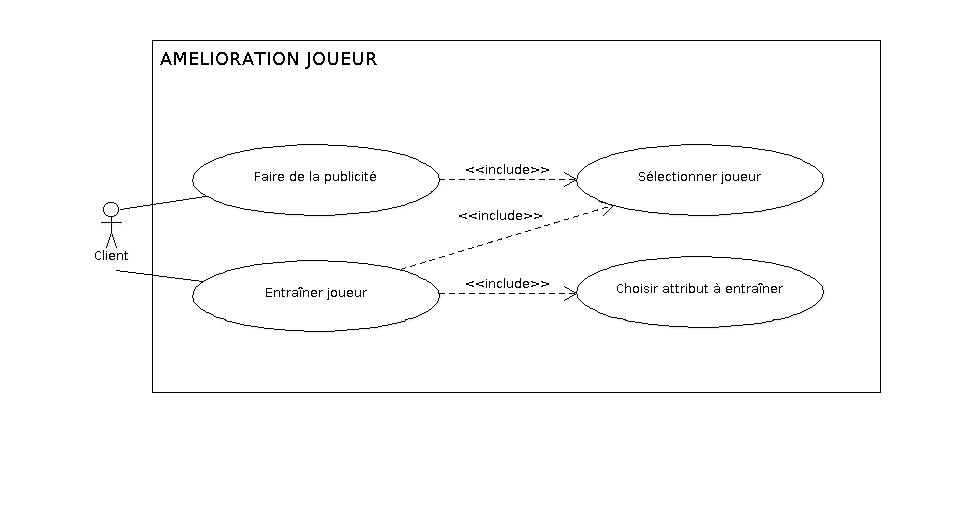
\includegraphics[scale=0.5]{uml/useCaseView/Ameliorationjoueur.png}
    \caption{Cas d'utilisation 6: Amélioration joueur}
  \end{figure}
  Lorsqu'il voudra augmenter les capacités de l'un de ses joueurs, 
  le Manager l'enverra au \enquote{\gls{centreentrainement}} \index{bâtiment!Centre d'entraînement}. 
  Une séance d'entraînement a un certain coût. 
  Ce coût varie en fonction du niveau d'entraînement déjà atteint par le joueur et en fonction du niveau du bâtiment.
  Le manager\index{manager} peut également améliorer la popularité d'un joueur en l'envoyant à l'\enquote{\gls{agencepublicite}} \index{bâtiment!Agence de publicité}. Encore une fois, le Manager doit payer pour bénéficier de ces services. Ces actions rendent le joueur indisponible jusqu'à la fin du temps requis pour réaliser l'entraînement ou la publicité.
    \subsubsection{Faire de la publicité}
      \begin{itemize}
        \item \textbf{Relations avec d'autres cas d'utilisation}  : Inclut Sélectionner joueur
        \item \textbf{Pré-conditions} : Le Manager dispose de suffisamment d’argent pour payer la publicité.
        \item \textbf{Post-conditions} : Le joueur est bloqué jusqu'à une certaine date sauvegardée dans un calendrier. Ce calendrier sera vérifié régulièrement.
        \item \textbf{Cas général} : Le Manager souhaite augmenter la popularité d'un joueur. Ceci est possible grâce au bâtiment \enquote{Agence de publicité}\index{bâtiment!Agence de publicité} dont le niveau détermine la durée. En payant une certaine somme, le client peut donc augmenter la popularité du joueur choisi. Le joueur est indisponible jusqu’à la fin de la publicité.

        \item \textbf{Cas exceptionnels} :
        \begin{itemize}
            \item Le Manager n'a pas les moyens de payer la publicité. Le programme le lui signale et l'action est annulée.
          \end{itemize}
      \end{itemize}
    \subsubsection{Entraîner joueur}
      \begin{itemize}
        \item \textbf{Relations avec d'autres cas d'utilisation}  : Inclut Sélectionner joueur et Choisir un attribut à entraîner.
        \item \textbf{Pré-conditions} : Le client dispose de suffisamment d’argent pour payer l’entraînement.
        \item \textbf{Post-conditions} : Le joueur est bloqué jusqu'à une certaine date sauvegardée dans un calendrier. Ce calendrier sera vérifié régulièrement.
        \item \textbf{Cas général} : Le client souhaite augmenter un attribut  d’un joueur. Le niveau du bâtiment concerné par cette action détermine la durée d'indisponibilité du joueur. En payant une certaine somme, le client peut donc augmenter une caractéristique du joueur choisi. En attendant la fin de l’entraînement, le joueur est donc indisponible.
        \item \textbf{Cas exceptionnels} :
        \begin{itemize}
            \item Le Manager n'a pas les moyens de payer la séance d'entraînement. Le programme le lui signale et l'action est annulée.
          \end{itemize}
      \end{itemize}
    \subsubsection{Sélectionner joueur}
      \begin{itemize}
        \item \textbf{Relations avec d'autres cas d'utilisation}  : Est inclus dans Faire de la publicité et Entraîner joueur
        \item \textbf{Pré-conditions} : Le joueur sélectionné doit être disponible ; c’est-à-dire qu’il ne peut être blessé (car il se trouverait alors à l'infirmerie), ni en train de faire un autre entraînement ou parti en campagne de promotion.
        \item \textbf{Post-conditions} : Le joueur sur lequel on va faire l’amélioration sera indisponible jusqu’à la fin de l’entraînement ou de la publicité.
        \item \textbf{Cas général} : Le Manager choisit de quel joueur il veut augmenter un attribut ou la popularité. 
        \item \textbf{Cas exceptionnels} : 
        \begin{itemize}
            \item Le joueur que le Manager désire sélectionner est momentanément indisponible (car en pleine séance d'entraînement, en campagne de promotion où est soigné à l'infirmerie). Le programme le lui signale et l'action est annulée.
          \end{itemize}
      \end{itemize}
    \subsubsection{Choisir attribut à entraîner}
      \begin{itemize}
        \item \textbf{Relations avec d'autres cas d'utilisation}  : Est inclus dans Entraîner joueur
        \item \textbf{Pré-conditions} : Le Manager a sélectionné un joueur et a décidé de l'entraîner.
        \item \textbf{Post-conditions} : L'attribut choisi sera augmenté lorsque la séance d'entraînement aura pris fin.
        \item \textbf{Cas général} : Le client choisit quel attribut il souhaite augmenter. Il ne peut entraîner qu’un attribut à la fois. 
        \item \textbf{Cas exceptionnels} :
        \begin{itemize}
            \item L'attribut choisi est déjà à son maximum. Le programme le lui signale et l'action est annulée.
          \end{itemize}
      \end{itemize}

  \subsection{Cas d'utilisation 7: le stade}
  \begin{figure}[H]
    \center
    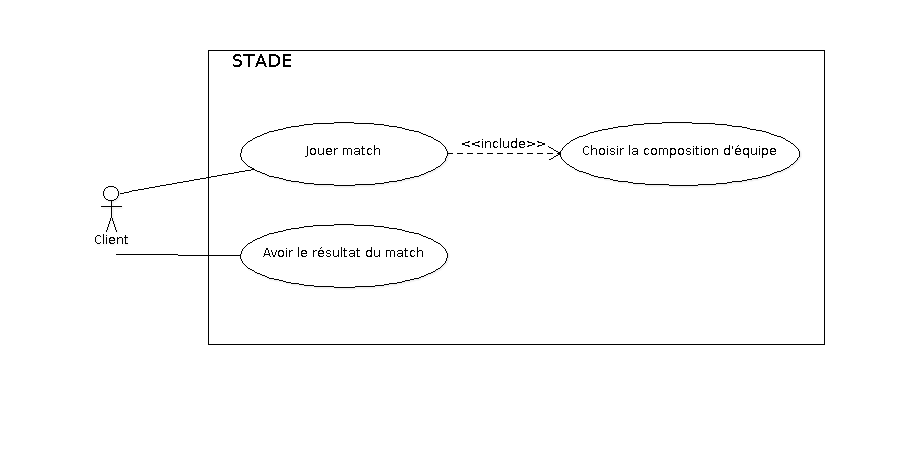
\includegraphics[scale=0.5]{uml/useCaseView/Stade.png}
    \caption{Cas d'utilisation 7: Stade}
  \end{figure}
  C'est via le \gls{stade} \index{bâtiment!Stade} que le Manager peut lancer un match lorsque c'est un jour de match. Il devra alors choisir les joueurs qui participeront à la rencontre. Une fois le match terminé, il pourra voir les résultats de ce dernier, ainsi que ce qu'il a gagné, ou perdu (argent et popularité).
    \subsubsection{Jouer match}
      \begin{itemize}
        \item \textbf{Relations avec d'autres cas d'utilisation}  : Inclut Choisir la composition d’équipe
        \item \textbf{Pré-conditions} : C’est un jour de match et l’adversaire est également connecté.
        \item \textbf{Post-conditions} : Il y a un gagnant et un perdant.
        \item \textbf{Cas général} : Pour savoir si c'est un jour de match, le programmme vérifie en checkant le \gls{calendrier} \index{calendrier} des matches. S'il y a bien un match de prévu, le Manager est connecté en même temps que son adversaire du jour. Ils doivent donc jouer le match dont la date a été prédéterminée.
        \item \textbf{Cas exceptionnels} : 
          \begin{itemize}
            \item L’adversaire ne se connecte jamais. Le Manager jouera contre l’équipe de son adversaire qui suivra une stratégie automatique minimaliste (Intelligence Artificielle).
          \end{itemize}
      \end{itemize}
    \subsubsection{Choisir la composition d'équipe}
      \begin{itemize}
        \item \textbf{Relations avec d'autres cas d'utilisation}  : Est inclus dans Jouer match
        \item \textbf{Pré-conditions} : Les joueurs choisis doivent être disponibles et être équipés d’un balai.
        \item \textbf{Post-conditions} : Néant.
        \item \textbf{Cas général} : Le client choisit les 7 \index{joueur}joueurs qui seront sur le \index{terrain}terrain pour le match qu’il doit jouer.
        \item \textbf{Cas exceptionnels} : 
        \begin{itemize}
            \item Le Manager n'en choisi aucun. 7 joueurs sont alors sélectionnés aléatoirement.
          \end{itemize}
      \end{itemize}
    \subsubsection{Avoir le résultat du match}
      \begin{itemize}
        \item \textbf{Relations avec d'autres cas d'utilisation}  : Néant.
        \item \textbf{Pré-conditions} : Le match doit être terminé.
        \item \textbf{Post-conditions} : Néant.
        \item \textbf{Cas général} : Après le match, le client peut voir le résultat du match et ce qui s’en suit ; l’argent gagné et l’effet sur la popularité des joueurs. 
        \item \textbf{Cas exceptionnels} : Néant.
      \end{itemize}

  
\section{Exigences non fonctionnelles}
  Pour le confort de l'utilisateur, il faudra  une interface graphique très intuitive, 
  les menus étant attachés à des  bâtiments, leur sélection par la souris ouvrira ces menus.
  De même, la gestion d'un match devra être aisée, malgré le nombre d'actions à choisir 
  sur un tour. Le plaisir de l'utilisateur apporté par le jeu dépendra du rythme de la succession de ces tours.
\section{Exigences de domaine}
  L'expérience immersive de l'utilisateur doit être connectée à l'univers fixé, 
  à savoir la saga d'Harry Potter. Cela signifie, d'une part, 
  qu'il ne faut pas contrevenir aux droits d'auteur portant sur les oeuvres 
  qui décrivent cet univers, et d'autre part, qu'il faut y ressembler suffisament pour que 
  l'utilisateur, familier de ce même univers, y retrouve les éléments le composant.
\chapter{Besoins du système}
  % Cette troisième section décrit en détail les fonctionnalités du
  % système (à partir de celles décrites à la section précédente), sans
  % aborder (dans la mesure du possible) *comment* elles doivent être
  % réalisées.
\section{Exigences fonctionnelles}
  % Ce type d’exigences sera décrit en utilisant des diagrammes use
  % case et en fournissant une description *plus détaillée* pour
  % chacun d’entre eux (comme vu au cours théorique et aux exercices).
 \subsection{Cas d'utilisation 1: Quidditch Manager 2014}
  \begin{figure}[H]
    \center
    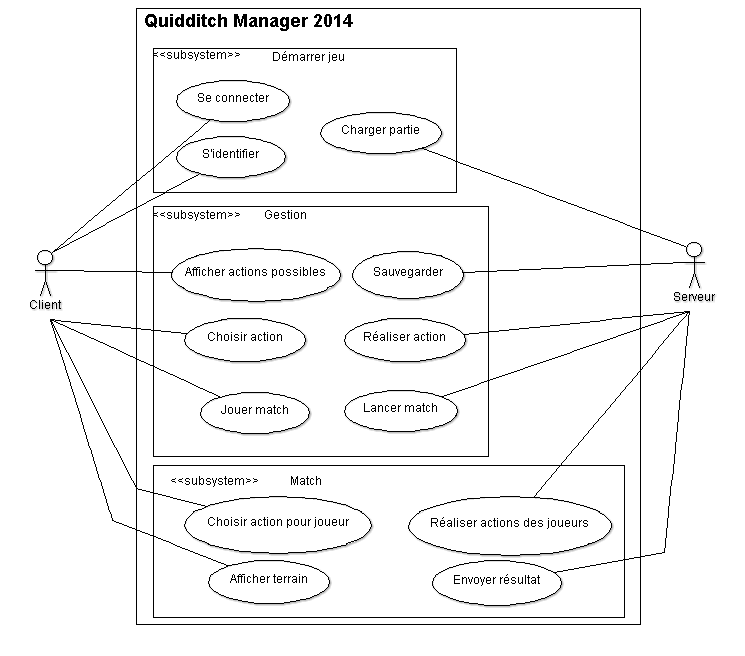
\includegraphics[scale=0.7]{uml/QM2014.png}
    \caption{Cas d'utilisation 1: Quidditch Manager 2014}
  \end{figure}	
    Ce diagramme représente le fonctionnement de base du jeu avec la répartition des "tâches" au niveau serveur et client.
    \subsubsection{Se connecter}
      \begin{itemize}
        \item \textbf{Acteur} : Client.
        \item \textbf{Relations avec d'autres cas d'utilisation}  : Néant.
        \item \textbf{Pré-conditions} : Le serveur doit être connecté.
        \item \textbf{Post-conditions} : Client et serveur sont reliés par le réseau.
        \item \textbf{Cas général} : Le client se connecte au serveur du jeu pour pouvoir jouer. 
        \item \textbf{Cas exceptionnels} : 
        \begin{itemize}
            \item La connexion au serveur échoue. Le programme le signale à l'utilisateur. Ceci termine ce use case.
          \end{itemize}
      \end{itemize}
    \subsubsection{S'identifier}
      \begin{itemize}
        \item \textbf{Acteur} : Client.
        \item \textbf{Relations avec d'autres cas d'utilisation}  : Néant.
        \item \textbf{Pré-conditions} : Le client est connecté au serveur.
        \item \textbf{Post-conditions} : Le client a accès à sa partie.
        \item \textbf{Cas général} : Le client crée une nouvelle \gls{partie}\index{partie} ou en charge une existante pour s’identifier auprès du serveur. Si le client charge une partie existante, le serveur va récupérer le fichier de sauvegarde approprié, sinon, il va en créer un nouveau.
        \item \textbf{Cas exceptionnels} : 
         \begin{itemize}
            \item Le client entre un identifiant ou un mot de passe déjà utilisé. Le programme le signale à l'utilisateur et lui redemande de s'identifier.
          \end{itemize}
      \end{itemize}
    \subsubsection{Charger partie}
      \begin{itemize}
        \item \textbf{Acteur}  : Serveur.
        \item \textbf{Relations avec d'autres cas d'utilisation}  : Néant.
        \item \textbf{Pré-conditions} : La connexion et l'authentification d'un client se sont déroulés sans encombre.
        \item \textbf{Post-conditions} : La partie est chargée.
        \item \textbf{Cas général} : Le serveur va charger les informations de la partie à laquelle va accéder le client.
        \item \textbf{Cas exceptionnels} : 
        \begin{itemize}
            \item Le client ne possède pas encore de partie. Le serveur lui en crée une.
          \end{itemize}
      \end{itemize}
    \subsubsection{Sauvegarder}
      \begin{itemize}
        \item \textbf{Acteur}  : Serveur.
        \item \textbf{Relations avec d'autres cas d'utilisation}  : Néant.
        \item \textbf{Pré-conditions} : Des informations relatives à la partie d'un client ont été modifiées et nécessitent d'être sauvées.
        \item \textbf{Post-conditions} : Les changements sont sauvegardés dans le fichier de sauvegarde dédié au client.
        \item \textbf{Cas général} : Le serveur sauvegarde les informations de la partie. L’état actuel de la partie du client est sauvegardée dans un fichier de sauvegarde.
        \item \textbf{Cas exceptionnels} : Néant.
      \end{itemize}
    \subsubsection{Afficher actions possibles}
      \begin{itemize}
        \item \textbf{Acteur}  : Client.
        \item \textbf{Relations avec d'autres cas d'utilisation}  : Néant.
        \item \textbf{Pré-conditions} : Le client est connecté au serveur.
        \item \textbf{Post-conditions} : Néant.
        \item \textbf{Cas général} : Le client affiche tout ce qu’il est possible de faire d’un point de vue gestion.
        \item \textbf{Cas exceptionnels} : Néant.
      \end{itemize}
    \subsubsection{Choisir action}
      \begin{itemize}
        \item \textbf{Acteur}  : Client.
        \item \textbf{Relations avec d'autres cas d'utilisation}  : Néant.
        \item \textbf{Pré-conditions} : Le client est connecté au serveur.
        \item \textbf{Post-conditions} : La requête a été envoyée au serveur.
        \item \textbf{Cas général} : Le client a choisi une action de gestion à effectuer (amélioration bâtiment, entraînement, publicité, achat, vente, gestion d’équipe). Il doit maintenant attendre que le serveur exécute cette action.
        \item \textbf{Cas exceptionnels} : 
        \begin{itemize}
            \item L'envoi échoue. Le programme le signale à l'utilisateur.
          \end{itemize}
      \end{itemize}
    \subsubsection{Réaliser action}
      \begin{itemize}
        \item \textbf{Acteur}  : Serveur.
        \item \textbf{Relations avec d'autres cas d'utilisation}  : Néant.
        \item \textbf{Pré-conditions} : Client et serveur sont connectés.
        \item \textbf{Post-conditions} : La requête a été traitée par le serveur.
        \item \textbf{Cas général} : Le client a choisi de faire une action de gestion (amélioration bâtiment, entraînement, publicité, achat, vente, gestion d’équipe). Le serveur va se charger de faire les modifications liées à cette action.
        \item \textbf{Cas exceptionnels} :
        \begin{itemize}
            \item La réception échoue. Le programme le signale à l'utilisateur.
          \end{itemize} 
      \end{itemize}
    \subsubsection{Jouer match}
      \begin{itemize}
        \item \textbf{Acteur}  : Client.
        \item \textbf{Relations avec d'autres cas d'utilisation}  : Néant.
        \item \textbf{Pré-conditions} : La date et le moment de la journée correspondent à un match prévu dans le championnat.
        \item \textbf{Post-conditions} : Ce \index{match}match est retiré du \gls{calendrier}\index{calendrier} des matches.
        \item \textbf{Cas général} : On va quitter la partie gestion pour lancer le match. Avant de pouvoir commencer le \index{match}match, le client doit choisir la liste des joueurs qui seront sur le terrain. 
        \item \textbf{Cas exceptionnels} : Néant.
      \end{itemize}
    \subsubsection{Lancer match}
      \begin{itemize}
        \item \textbf{Acteur}  : Serveur.
        \item \textbf{Relations avec d'autres cas d'utilisation}  : Néant.
        \item \textbf{Pré-conditions} : Au moins un des clients qui doivent s’affronter lors de ce match est connecté.
        \item \textbf{Post-conditions} : Néant.
        \item \textbf{Cas général} : Le serveur va maintenant gérer le match et l’aspect gestion ne sera plus accessible tant que le match ne sera pas terminé.
        \item \textbf{Cas exceptionnels} : 
          \begin{itemize}
            \item Un des clients ne s’est pas connecté pour le match, le serveur prendra sa place pour déplacer ses joueurs et affronter le client connecté.
			\item Aucun client ne s’est connecté pour le match, le match est considéré comme annulé.
          \end{itemize}    	
      \end{itemize}
    \subsubsection{Choisir action pour joueur}
      \begin{itemize}
        \item \textbf{Acteur}  : Client.
        \item \textbf{Relations avec d'autres cas d'utilisation}  : Néant.
        \item \textbf{Pré-conditions} : Le joueur sélectionné est encore libre de faire une action.
        \item \textbf{Post-conditions} : L'action choisie est réalisée par ce joueur lors du tour.
        \item \textbf{Cas général} : Le client choisit l'action que devra réaliser le joueur lors du tour. Cela peut-être un déplacement et/ou une action particulière comme passer le \index{balle!souafle}souafle ou tirer aux buts. Le client doit faire cela pour chacun de ses joueurs ou indiquer au serveur qu’il a fini de choisir ses actions (s’il souhaite par exemple que des joueurs ne fassent rien).
        \item \textbf{Cas exceptionnels} : 
        \begin{itemize}
         \item Le client ne donne aucune instruction au joueur. Le joueur reste sur place.
        \end{itemize}
      \end{itemize}
    \subsubsection{Réaliser action des joueurs}
      \begin{itemize}
        \item \textbf{Acteur}  : Serveur.
        \item \textbf{Relations avec d'autres cas d'utilisation}  : Néant.
        \item \textbf{Pré-conditions} : Cette action se déroule dans le cadre d'un match.
        \item \textbf{Post-conditions} : La situation sur le terrain a évolué.
        \item \textbf{Cas général} : A chaque tour, le serveur attend de recevoir les actions que les clients ont choisies pour chacun de leurs joueurs. Une fois l’ensemble de ces actions reçues, le serveur les exécute puis envoie la nouvelle situation aux clients. Les clients affichent alors le terrain et redemandent les actions à exécuter aux utilisateurs.
        \item \textbf{Cas exceptionnels} : 
          \begin{itemize}
            \item Si un des clients ne s’est pas connecté pour le match, le serveur n’attendra pas d’actions de la part de ce client. Ses joueurs suivront une stratégie automatique minimaliste prise en charge par le serveur.
          \end{itemize}  
      \end{itemize}
    \subsubsection{Afficher terrain}
      \begin{itemize}
        \item \textbf{Acteur}  : Client.
        \item \textbf{Relations avec d'autres cas d'utilisation}  : Néant.
        \item \textbf{Pré-conditions} : Le client est connecté au serveur et un match a lieu.
        \item \textbf{Post-conditions} : Néant.
        \item \textbf{Cas général} : Le client reçoit les informations relatives au \index{terrain}terrain de la part du serveur et l’affiche pour permettre au client de facilement visualiser la situation actuelle du jeu.
        \item \textbf{Cas exceptionnels} : Néant. 
      \end{itemize}
    \subsubsection{Envoyer résultat}
      \begin{itemize}
        \item \textbf{Acteur}  : Serveur.
        \item \textbf{Relations avec d'autres cas d'utilisation}  : Néant.
        \item \textbf{Pré-conditions} : Le match est terminé.
        \item \textbf{Post-conditions} : Le client dispose des informations à afficher après un match.
        \item \textbf{Cas général} : Le match est terminé. Le serveur va calculer combien le Manager a gagné (en fonction des bâtiments \gls{fanshop}\index{bâtiment!FanShop} (match à domicile) ou \gls{buvette}\index{bâtiment!Buvette} (match en extérieur)). En fonction de la situation de fin de match, victoire ou défaite, le serveur va également déterminer combien d’argent et de popularité le Manager a gagné ou perdu. Toutes ses informations sont envoyées au client.
        \item \textbf{Cas exceptionnels} : Néant.
      \end{itemize}




\section{Exigences non fonctionnelles}
  \subsection{Le réseau}
  Au niveau du réseau, le problème de la synchronisation n'est pas préoccupant, 
  car le client ne sera qu'une interface d'affichage et d'interaction. 
  Pour ce qui est de la quantité d'informations échangées, 
  elle ne devrait pas être très importante pour autant, 
  les éléments à afficher et leur diversité étant relativement réduits.
  
  Il faudra veiller à ce que l'interaction avec l'utilisateur soit transparente 
  au niveau du serveur, à travers une classe de message générique, 
  que le programme client instanciera de la même manière, 
  qu'il tourne à travers une interface graphique ou à travers le terminal.
  \subsection{Performance}
  Pour ce qui est de la performance, la localisation de tous les calculs sur la machine serveur 
  implique une centralisation de la puissance de calcul. 
  D'un autre côté, le client ne nécessitera que très peu de puissance de son côté pour pouvoir jouer.
  \subsection{Sécurité}
  La sécurité d'une partie sera assurée par l'identification : 
  seul un utilisateur identifié peut charger une partie, et la sienne uniquement.
  \subsection{Environnement d'exécution}
  L'environement d'exécution étant fixé (les machines des salles informatiques du NO), 
  le code se limitera à l'utilisation des librairies C++ standards. 
  Le système d'exploitation visé est GNU/Linux.
\section{Design et fonctionnement du système}
  % Cette partie sera décrite à l’aide des différents diagrammes UML
  % vus au cours théorique et aux exercices.
  \subsection{Diagrammes de classes}
  Nous allons ici présenter les différentes classes et leurs relations.
    \begin{figure}[H]
    \center
    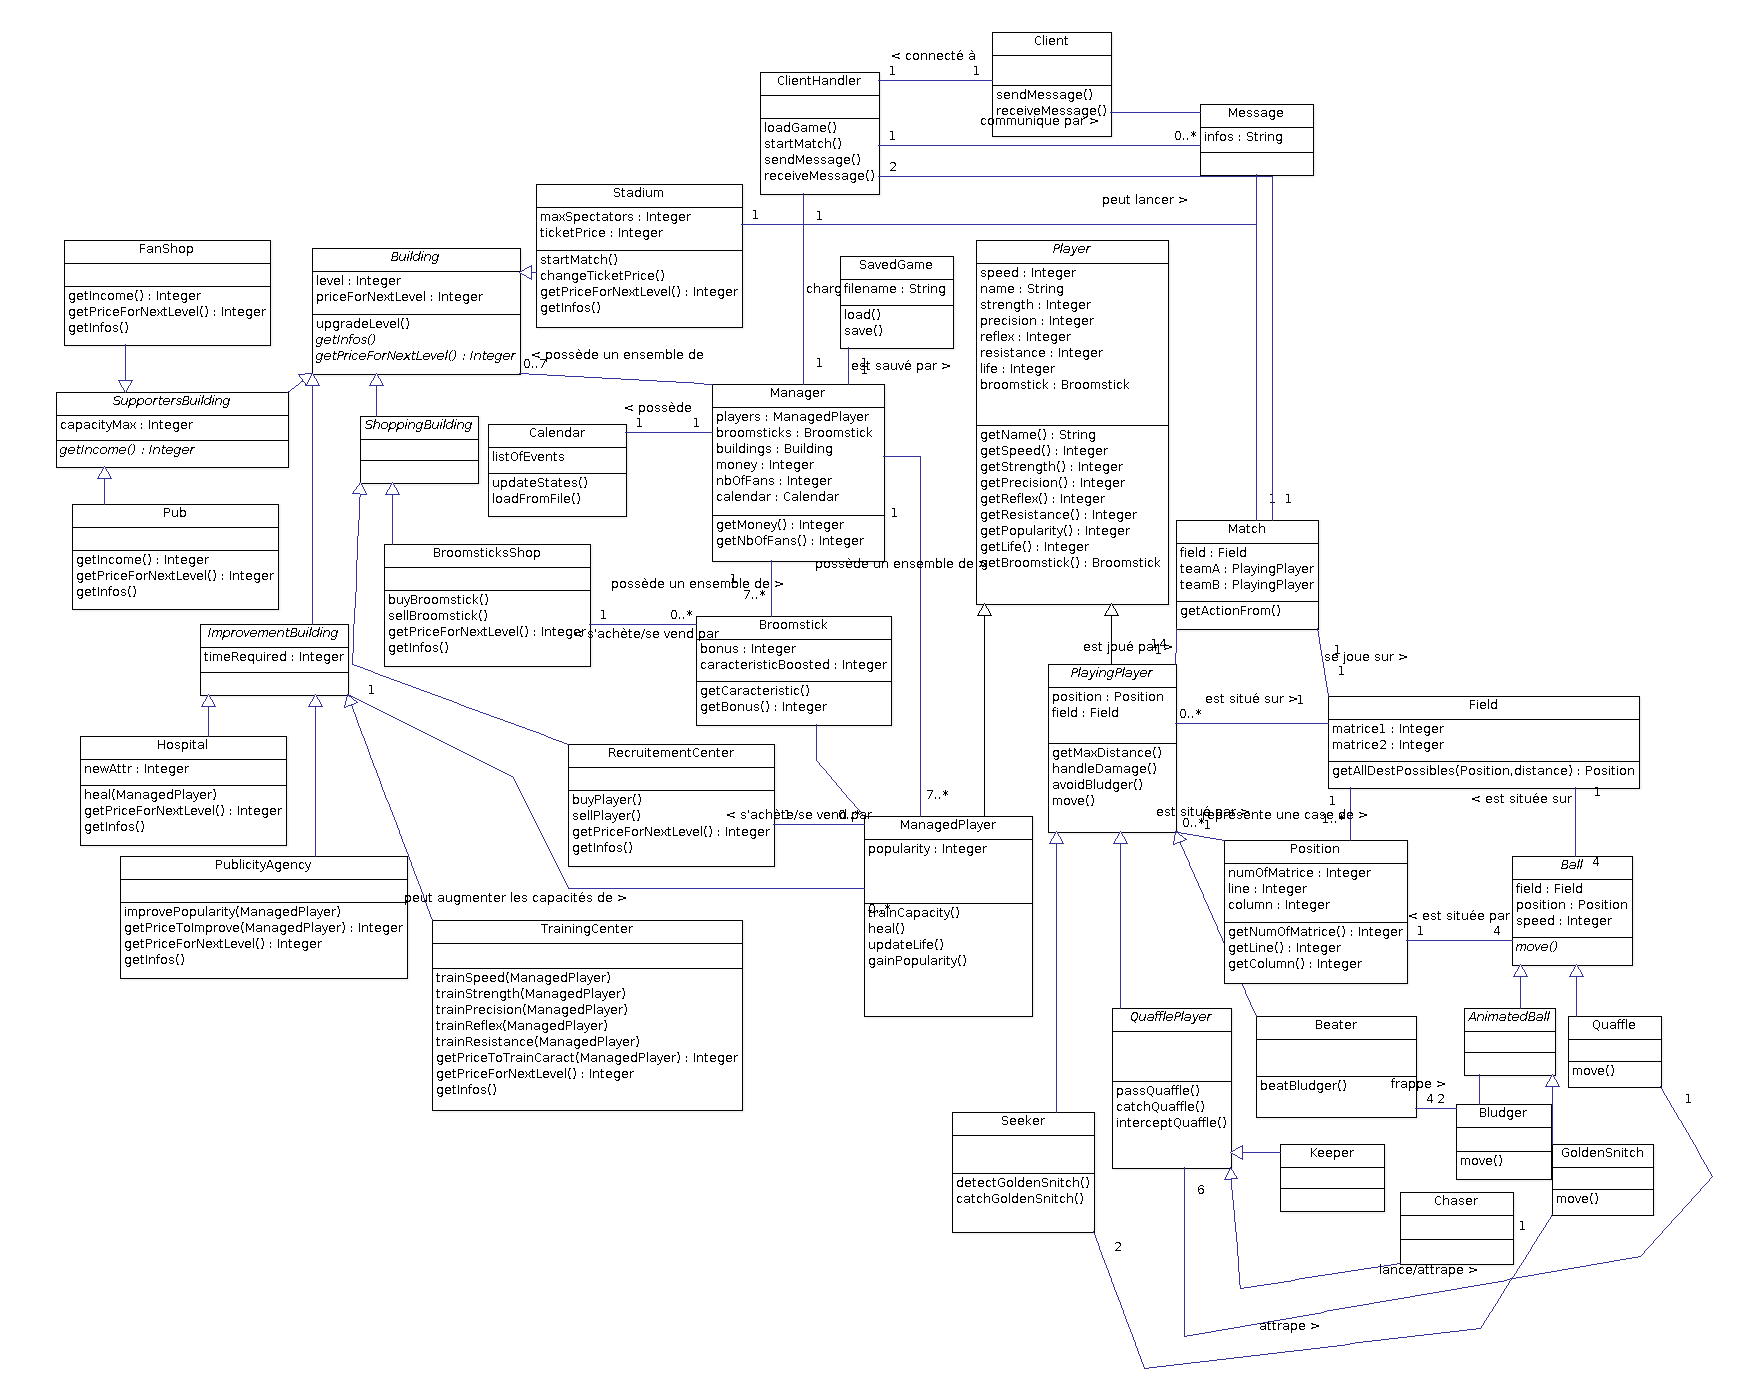
\includegraphics[scale=0.3]{uml/class/ClassDiagram.png}
    \caption{Diagramme de classe général}
  \end{figure}	
  \subsubsection{Les joueurs}
    \begin{figure}[H]
    \center
    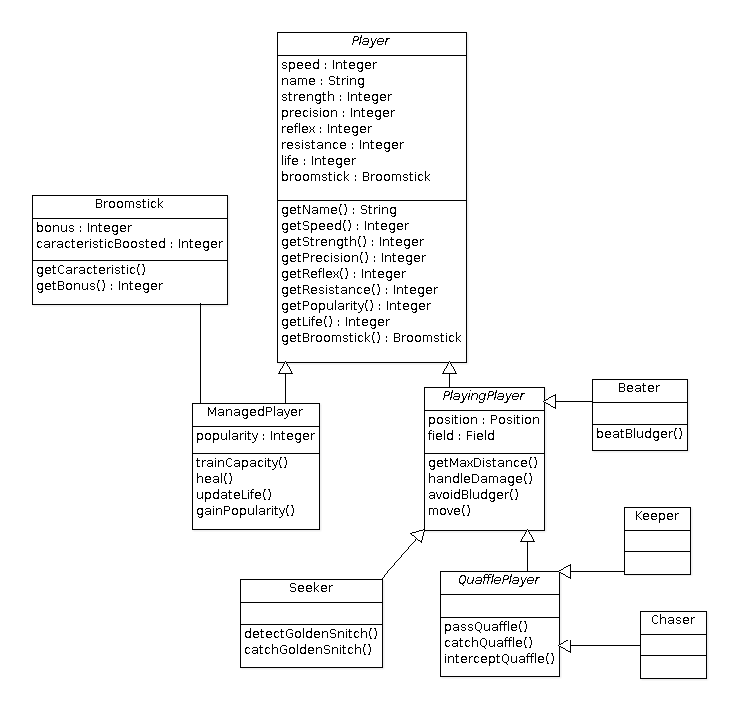
\includegraphics[scale=0.4]{uml/class/DiagrammedeclassesJoueurs.png}
    \caption{Diagramme des classes joueurs}
  \end{figure}	
    Une classe abstraite réprésente le \gls{joueur}\index{joueur} avec ses caractéristiques de base.
    Dans un soucis de découplage, nous différencions deux classes spécialisées à partir de cette base.
    Le joueur au niveau de la gestion est distingué du joueur au niveau du match\index{match}.
    En effet, ils nécessitent chacun des méthodes fort différentes :
    d'un côté des méthodes d'amélioration d'attributs,
    de l'autre des méthodes d'actions spécifiques à un match.
    Les attributs du joueur de match, ce dernier pouvant se construire depuis un joueur
    au niveau de la gestion, ne sont pas une simple transposition des caractéristiques
    du joueur en gestion. En effet, intervient notamment le calcul du bonus lié au balai.
  \subsubsection{Concernant le réseau}
    \begin{figure}[H]
    \center
    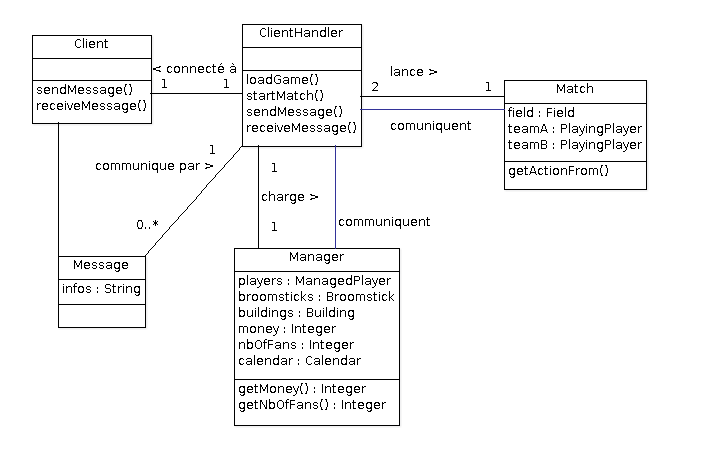
\includegraphics[scale=0.5]{uml/class/Diagrammedeclasses.png}
    \caption{Diagramme des classes impliquées dans le réseau}
    \end{figure}	
    La relation avec le client est gérée par une classe principale, qui va assurer la communication
    à travers une classe de messages (un \emph{struct} puisque la base réseau sera écrite en C).
    C'est cette classe principale qui va gérer les alternances entre le côté gestion et le côté match. Le match nécessite une connexion entre deux clients, elle est donc très différente de la gestion
    à ce niveau-là aussi.
  \subsubsection{Concernant la gestion générale}
    \begin{figure}[H]
    \center
    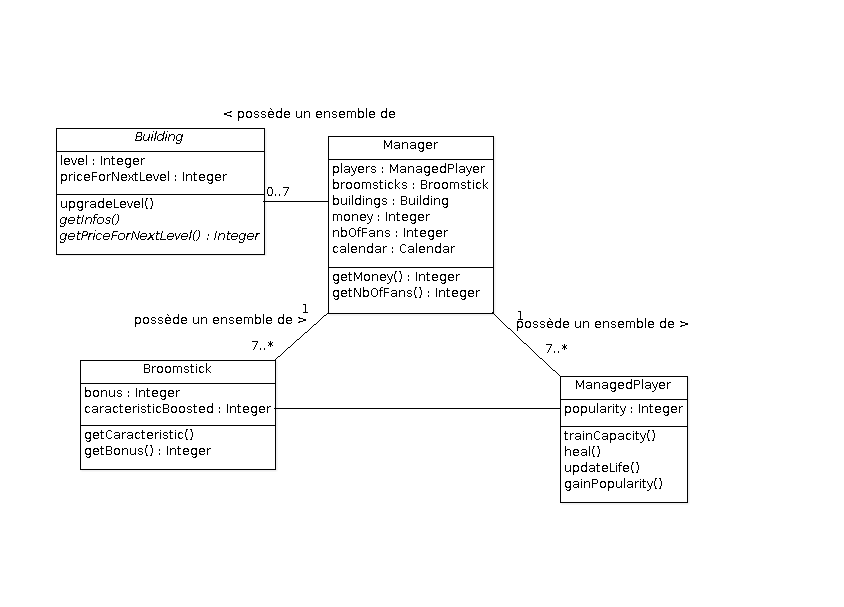
\includegraphics[scale=0.5]{uml/class/DiagrammedeclassesManagement.png}
    \caption{Diagramme des classes impliquées dans la partie gestion}
    \end{figure}	
    Le manager est la classe dédiée à la partie gestion. Elle représente une partie du jeu,
    composée d'un ensemble de joueurs\index{joueur}, de balais\index{balai}, de bâtiments\index{bâtiment}, d'un calendrier\index{calendrier} et d'un trésor\index{trésor}.
    Elle donne accès aux bâtiments qui chacun donne accès aux possibilités d'améliorations, d'achats et de vente.
  \subsubsection{Concernant le match}
    \begin{figure}[H]
    \center
    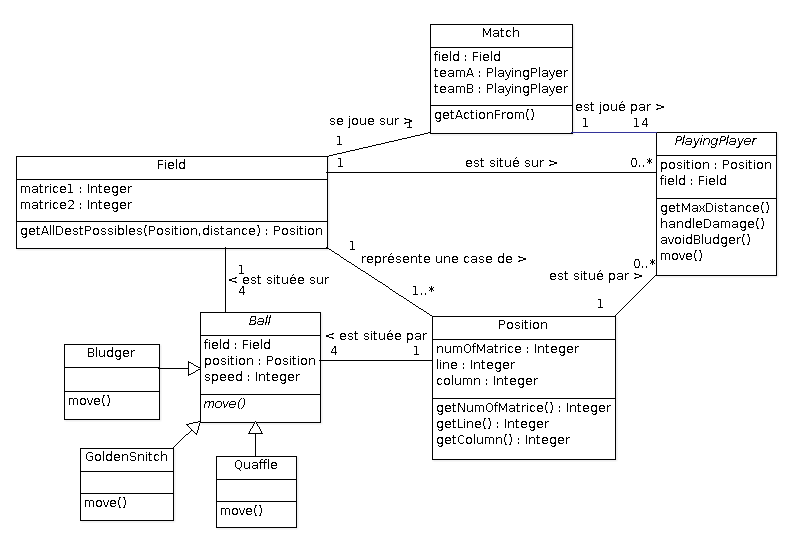
\includegraphics[scale=0.4]{uml/class/Diagrammedeclassesmatch.png}
    \caption{Diagramme des classes impliquées dans les matchs}
    \end{figure}	
    Le match relie deux clients différents dans un affrontement sur un \gls{terrain}\index{terrain} 
    où se déplacent à la fois des joueurs et des \index{balle}balles, les joueurs pouvant faire se déplacer les balles. La classe \emph{Position} regroupe les informations de position d'un joueur ou d'une balle sur le terrain.
  \subsubsection{Les bâtiments}
    \begin{figure}[H]
    \center
    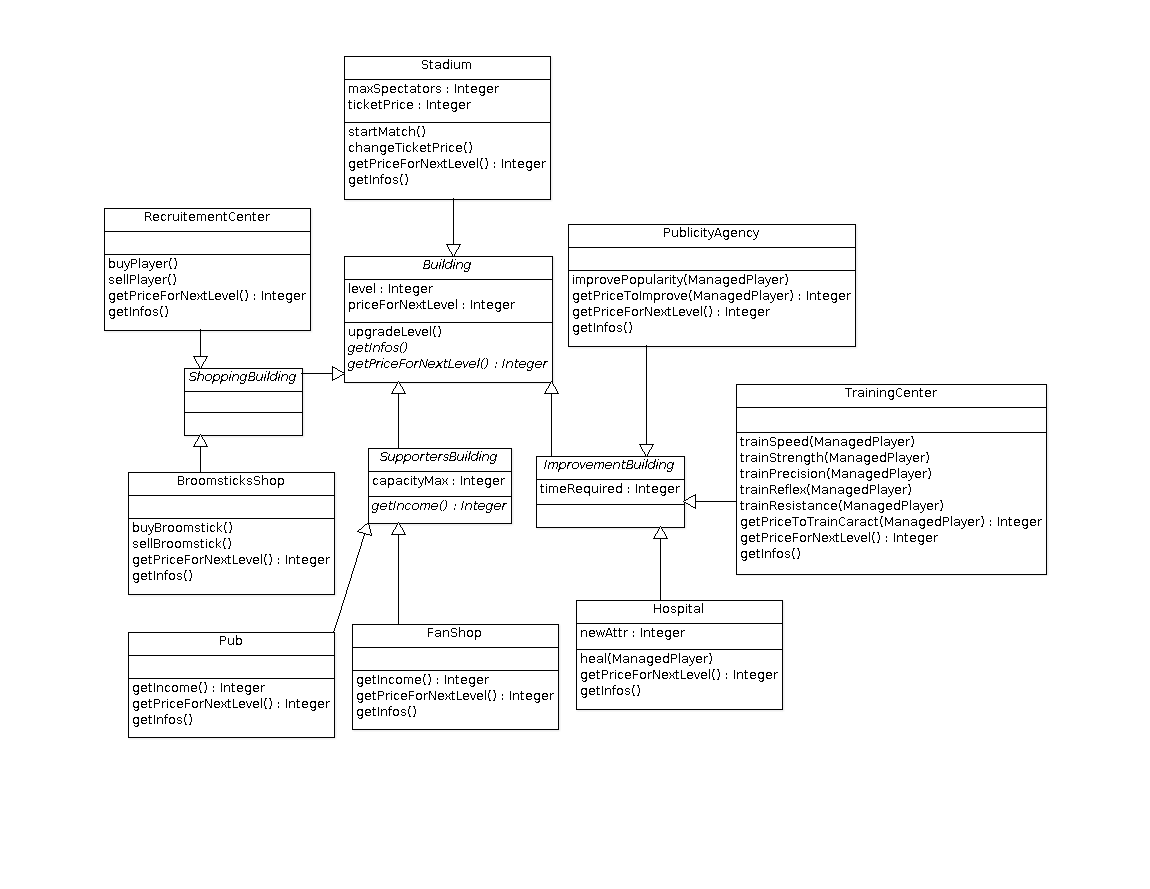
\includegraphics[scale=0.4]{uml/class/DiagrammedeclassesBuildings.png}
    \caption{Diagramme des classes de bâtiments}
    \end{figure}	
  Une classe abstraite représente tout bâtiment. Cette classe est dérivée dans d'autres classes abstraites
  qui regroupent les types de bâtiments\index{bâtiment} selon leur rôle principal (achat/vente, augmentation
  d'une capacité), plus le stade\index{bâtiment!Stade} à partir duquel un nouveau match peut démarrer. Par exemple, l'\gls{infirmerie}\index{bâtiment!infirmerie} fait partie des bâtiments
  améliorant les joueurs puisqu'elle soigne leurs blessures.
  Les attributs communs sont le niveau (chaque bâtiment à un niveau, le niveau 0
  signifiant \enquote{pas encore construit}) ainsi que le prix pour passer au niveau suivant.
  \subsubsection{Concernant les fichiers}
    \begin{figure}[H]
    \center
    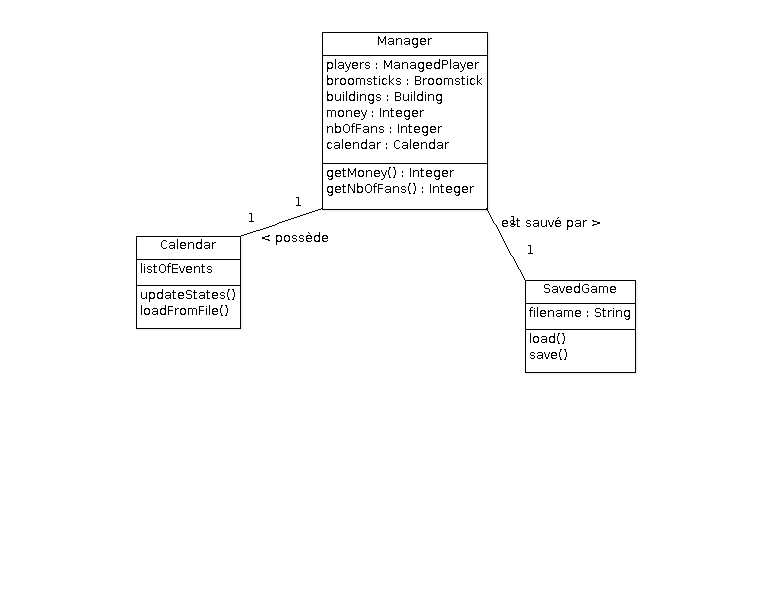
\includegraphics[scale=0.4]{uml/class/Fichiers.png}
    \caption{Diagramme des classes impliquées dans l'enregistrement}
    \end{figure}	
  L'état d'une partie aussi bien que les actions bloquantes ou planifiées doivent
  être enregistrées pour perdurer entre deux connexions. Pour cela, nous utilisons
  deux classes qui vont permettre de charger des données depuis le disque ou
  de les y sauvegarder.
  \subsection{Diagramme de séquence}
  Voici un diagramme de séquence qui illustre la gestion des différents
  rôles du serveur au travers de différents processus.
    \begin{figure}[H]
    \center
    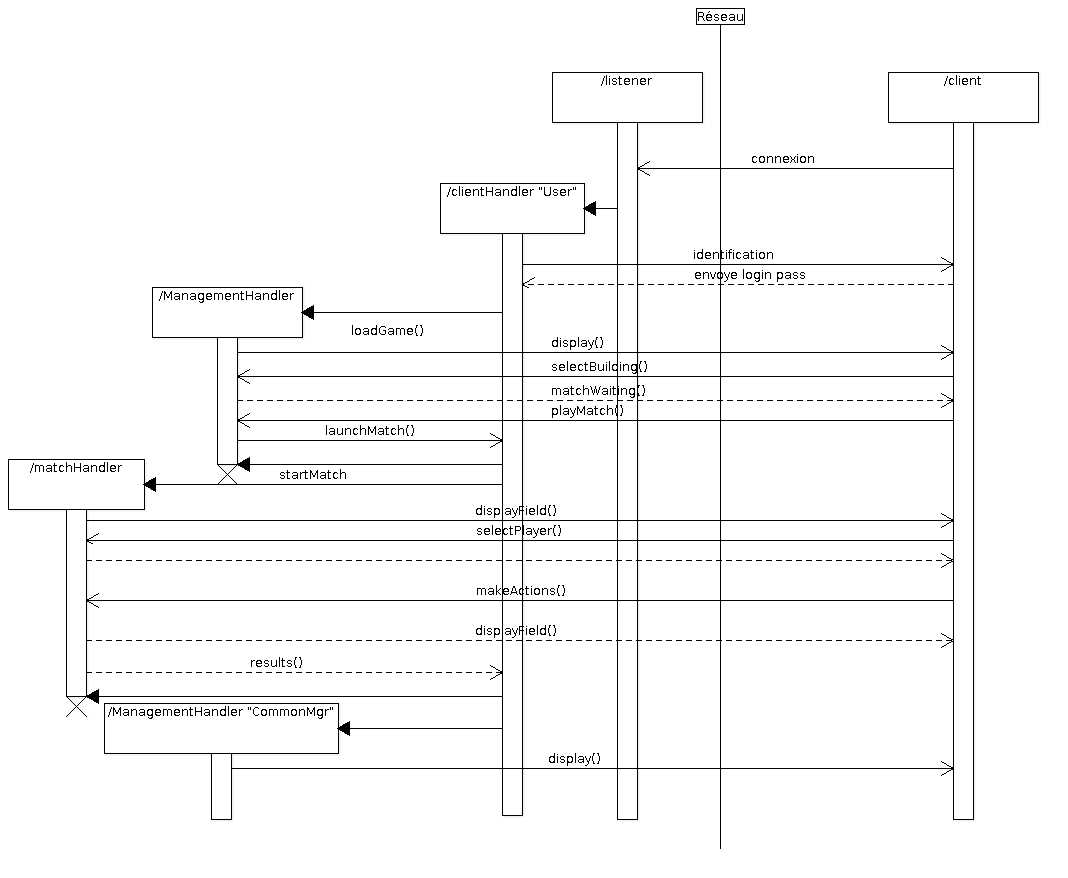
\includegraphics[scale=0.4]{uml/class/connexionserveurclient.png}
    \caption{Diagramme des classes impliquées dans le réseau}
    \end{figure}	
  Le côté gestion est bien dissocié du côté match, et le \emph{clientHandler} assure la communication avec le client.
  C'est le \emph{clientHandler} du manager\index{manager} qui reçoit le match dans son stade
  qui va créer l'instance en charge du match.
    

%\chapter{Index des termes utilisés}
%  Contiendra, au moins, toutes les entrées du glossaire (avec les numéros des pages correspondantes).
\addcontentsline{toc}{chapter}{4 Index}
\phantomsection
\printindex

\end{document}
